\documentclass[USenglish]{article}

\usepackage[utf8]{inputenc}
\usepackage{xparse}
\usepackage[big,online]{dgruyter}
\usepackage{lmodern}
\usepackage{microtype}
\usepackage[authoryear,round,sort&compress]{natbib}
\usepackage{graphicx}
\usepackage{booktabs}
\usepackage{multirow}
\usepackage{array}

\theoremstyle{dgthm}
\newtheorem{theorem}{Theorem}
\newtheorem{corollary}{Corollary}
\newtheorem{proposition}{Proposition}
\newtheorem{lemma}{Lemma}

\theoremstyle{dgdef}
\newtheorem{definition}{Definition}
\newtheorem{example}{Example}
\newtheorem{remark}{Remark}

\begin{document}

%%%--------------------------------------------%%%
\articletype{Research Article}
\received{October DD, 2025}
\revised{February DD, 2026}
\accepted{Month DD, YYYY}
\journalname{Journal of Quantitative Analysis in Sports}
\journalyear{YYYY}
\journalvolume{XX}
\journalissue{X}
\startpage{1}
\aop
\DOI{10.1515/jqas-YYYY-XXXX}
%%%--------------------------------------------%%%

\title{Coach WAR: A Counterfactual Approach to Evaluating NFL Head Coach Impact in the Modern Era}
\runningtitle{Coach WAR: Evaluating NFL Head Coach Impact}

% Author information removed for blind peer review
%\author*[1]{Jon Williamson}
%\runningauthor{J.~Williamson}
%\affil[1]{\protect\raggedright
%Des Moines, Iowa, e-mail: jon@williamsonconsultinggroup.com}

\abstract{Evaluating NFL head coach performance is challenging due to complex interactions among coaching decisions, player talent, and organizational factors. We introduce a counterfactual framework measuring head coach impact by predicting team performance under a replacement-level coach, then comparing this baseline to actual results. This difference represents coaching Wins Above Replacement (WAR). Analyzing 1,637 team-seasons (1970--2024) with 365 features spanning draft history, injuries, rosters, team performance, and coaching histories, we employ XGBoost regression to isolate coaching contributions from team context. The model achieves test $R^2 = 0.616$ on held-out coaches, with a residual standard error of $\pm$2.0 wins per season. Results indicate meaningful variation in coaching impact: elite coaches average up to +2.4 WAR per season (95\% CI: [+0.9, +3.9]) while the poorest coaches average $-$3.5 WAR (95\% CI: [$-$4.7, $-$2.3]). Offensive versus defensive coaching backgrounds show a historical shift---defensive coaches held a significant advantage in the 1970s ($-$0.87, 95\% CI: [$-$1.45, $-$0.29], $p = 0.005$), while offensive coaches now hold a +0.59 edge in the 2020s (95\% CI: [$-$0.05, +1.24], $p = 0.11$). Year-to-year persistence analysis reveals low stability, with WAR explaining only 7.3\% of next-season variance and offensive coaches showing significantly less multi-year persistence than defensive coaches ($p = 0.009$).}

\keywords{coaching analytics, wins above replacement, NFL, sports analytics}

\maketitle

\section{Introduction}

Evaluating head coach performance in the National Football League (NFL) presents unique challenges due to complex interactions among coaching decisions, player talent, and organizational factors. Traditional metrics such as win--loss records conflate team success with coaching quality, failing to isolate a coach's contribution from the context in which that coach operates.

We propose a counterfactual framework for measuring head coach impact: for each team-season, we predict how the team would have performed under a replacement-level coach with league-median characteristics, then compare this prediction to actual results. The difference represents coaching Wins Above Replacement (WAR). By controlling for roster quality, strength of schedule, salary allocation, injury exposure, and other contextual factors, the framework isolates the coaching contribution from the surrounding talent and organizational context.

\section{Literature Review}

Prior research on coaching evaluation has taken several approaches. \citet{hadley2000} used a Poisson regression framework with basic team statistics to assess NFL coaching efficiency relative to production frontiers, while \citet{goff2006} examined managerial lifecycle effects. The present work expands on \citet{hadley2000} by isolating coaching impact from a broader set of contextual factors, including salary distribution, player turnover, injury data, and detailed coach-specific performance histories.

WAR methodologies for player evaluation are well established in baseball \citep{palmer1984,smith2008,woolner2002} and have been extended with formal uncertainty quantification. \citet{baumer2015} developed openWAR with resampling-based interval estimates, advocating for uncertainty quantification as standard practice in WAR metrics. \citet{brill2024} proposed Grid WAR as an alternative aggregation for pitchers, further demonstrating the importance of methodological choices in WAR construction. In football, \citet{yurko2019} introduced nflWAR for offensive player evaluation, and \citet{sabin2021} estimated player value using plus--minus models that isolate individual contributions within a team sport.

Tree-based machine learning methods have proven effective for NFL prediction tasks. \citet{lock2014} used random forests to estimate within-game win probability, demonstrating the effectiveness of ensemble tree methods for NFL prediction tasks. More broadly, the growth of NFL tracking data has expanded the scope of quantitative football research \citep{lopez2020}. In basketball, \citet{deshpande2016} estimated individual player impact on team winning probability, addressing challenges of attribution in team sports that parallel those in coaching evaluation.

Our contribution extends the WAR framework to coaching evaluation, adapting the counterfactual approach to isolate coaching impact in a setting where coaches influence outcomes indirectly through strategic and personnel decisions rather than direct play execution.

\section{Methods}

\subsection{Data Sources and Feature Engineering}

We analyzed 1,637 team-seasons spanning 1970--2024, representing all 32 current NFL franchises across the Modern Era of professional football. The analysis incorporated 365 features from multiple data sources: draft pick history, injury reports, starter designations, complete rosters, historical team performance, and comprehensive head coach career histories from Pro Football Reference, along with salary cap allocation and contract details from Spotrac. Feature counts by category are shown in Appendix A (Table~\ref{tab:feature_counts}).

The coach-specific feature set comprised 139 features in three groups: (1)~seven coaching experience variables (years of NFL and college experience as position coach, coordinator, or head coach, plus number of prior head coaching hires); (2)~66 normalized team performance statistics from the coach's most recent offensive or defensive coordinator tenure; and (3)~66 normalized opponent performance statistics from the coach's head coaching history. All performance features were z-score normalized within each season to ensure cross-era comparability. Non-coaching features captured roster construction (turnover rates, player age and experience by position), financial management (salary cap allocation percentages), injury exposure (games missed by starters), draft capital investment, and team performance context (strength of schedule, penalty rates). Data availability varied by category: team performance and roster metrics extended across all seasons, while salary cap data was limited to 2011--2024 and player injury data to 2009--2024.

\subsection{The Counterfactual Framework}

To isolate coaching impact from roster quality, organizational context, and other factors, we developed a counterfactual approach: for each team-season, we predict what the team's performance would have been under a replacement-level coach with league-median coaching characteristics, then compare this prediction to actual results.

Formally, let $\mathbf{x}_i = (\mathbf{x}_i^{(c)}, \mathbf{x}_i^{(t)})$ denote the feature vector for team-season $i$, where $\mathbf{x}_i^{(c)} \in \mathbb{R}^{139}$ are coaching features and $\mathbf{x}_i^{(t)} \in \mathbb{R}^{226}$ are non-coaching features. We compute replacement-level coaching features $\tilde{\mathbf{x}}^{(c)}$ as follows: for each coach $j$, we first compute the career mean $\bar{\mathbf{x}}_j^{(c)}$ across all of coach $j$'s seasons, then take the component-wise median across all coaches:
\begin{equation}
\tilde{x}^{(c)}_k = \operatorname{median}_j\!\bigl(\bar{x}_{j,k}^{(c)}\bigr), \quad k = 1, \ldots, 139.
\label{eq:replacement}
\end{equation}
This two-stage aggregation ensures each coach is weighted equally regardless of tenure length. The replacement-level prediction is then $\hat{y}_i^{(r)} = f(\tilde{\mathbf{x}}^{(c)}, \mathbf{x}_i^{(t)})$, where $f$ is the trained model.

This approach parallels established WAR methodologies in baseball \citep{palmer1984,woolner2002,baumer2015,yurko2019} and basketball \citep{berri2006,deshpande2016}, where player contributions are measured against replacement-level alternatives. Unlike baseball's replacement level, set at a .294 winning percentage representing readily available minor league talent \citep{appelman2013,baseballref_war}, we define replacement-level coaching as the league median. This choice reflects the coaching labor market's structure: NFL head coaches average only 3.2 years of tenure \citep{goff2006}, substantially shorter than MLB players' average career of 5.6 years \citep{witnauer2007}, making the median coach a more appropriate baseline than a theoretical minimum-quality hire.

\subsection{Model Specification}

We employed XGBoost \citep{chen2016}, a gradient-boosted regression tree ensemble that minimizes the regularized objective
\begin{equation}
\mathcal{L} = \sum_{i=1}^{n} \ell\!\bigl(y_i, \hat{y}_i\bigr) + \sum_{m=1}^{M} \Omega(f_m), \quad \Omega(f) = \gamma T + \tfrac{1}{2}\lambda \|w\|^2 + \alpha \|w\|_1,
\label{eq:xgboost}
\end{equation}
where $\ell$ is the squared-error loss, $T$ is the number of leaves in tree $f$, $w$ are leaf weights, and $\gamma$, $\lambda$, $\alpha$ are regularization parameters. XGBoost was selected for its ability to capture non-linear relationships and feature interactions while providing interpretable feature importance metrics, properties also leveraged in NFL analytics by \citet{lock2014} for win probability estimation.

Missing values arising from incomplete early-era salary and injury data were imputed via truncated Singular Value Decomposition (SVD) matrix completion \citep{brand2002}. We retained $k = 10$ singular components (capturing $>$90\% of observed variance), iterated until convergence (tolerance $10^{-4}$), and standardized non-normalized features prior to imputation to prevent scale-dependent bias.

To prevent data leakage, we employed coach-based train/test stratification: 216 coaches and all their associated seasons were assigned to the training set (81.7\% of observations), while 54 held-out coaches formed the test set (18.3\%). This ensures the model's test performance reflects generalization to entirely unseen coaching tenures. Hyperparameters were selected via randomized search over a discrete grid with 200 iterations and 5-fold cross-validation on the training set, optimizing $R^2$. Final hyperparameter values are shown in Appendix~B (Table~\ref{tab:hyperparameters}).

\subsection{WAR Calculation}

Coach WAR is computed as the difference between actual winning percentage and the replacement-level prediction, scaled to a 16-game season:
\begin{equation}
\text{WAR}_i = 16 \times \bigl(y_i - \hat{y}_i^{(r)}\bigr),
\label{eq:war}
\end{equation}
where $y_i$ is the actual winning percentage and $\hat{y}_i^{(r)} = f(\tilde{\mathbf{x}}^{(c)}, \mathbf{x}_i^{(t)})$ is the replacement-level prediction from Equation~\ref{eq:replacement}. All WAR calculations are standardized to a 16-game season, including the 17-game seasons beginning in 2021, to ensure cross-era comparability and prevent artificial inflation of recent values. For 17-game seasons, this represents a 6\% conservative adjustment.

\subsection{Uncertainty Quantification}

As advocated by \citet{baumer2015} for player WAR, we report interval estimates alongside point estimates. Because coaching WAR is observed at the season level without sub-seasonal granularity, we use analytical $t$-intervals on each coach's season-level WAR values rather than the bootstrap resampling approach used for play-level player metrics. We quantify uncertainty at three levels.

\textit{Career WAR confidence intervals.} For coach $c$ with $n_c$ seasons of individual WAR values $\{w_{c,1}, \ldots, w_{c,n_c}\}$, the career average WAR and its 95\% confidence interval are
\begin{equation}
\overline{w}_c \pm t_{n_c-1,\,0.025} \cdot \frac{s_c}{\sqrt{n_c}},
\label{eq:career_ci}
\end{equation}
where $s_c$ is the sample standard deviation of individual-season WAR values and $t_{n_c-1,\,0.025}$ is the critical value from the $t$-distribution with $n_c - 1$ degrees of freedom. These intervals directly address career sample size: coaches with few seasons (e.g., $n_c = 3$) produce wide intervals, while long-tenured coaches yield narrow intervals.

\textit{Single-season precision.} We report the model residual standard error, computed as the root mean squared error on the held-out coach test set converted to a 16-game season scale: $\text{SE}_{\text{model}} = 16 \times \text{RMSE}_{\text{test}}$. This provides a global measure of single-season WAR precision applicable to all observations.

\textit{Group comparison intervals.} For offensive-versus-defensive coaching background comparisons, we report Welch's $t$-interval on the difference in group means with Welch--Satterthwaite degrees of freedom, alongside Mann--Whitney $U$ tests for non-parametric confirmation. All correlation comparisons (e.g., persistence differences between coaching backgrounds) use Fisher's $Z$-transformation. All $p$-values are two-sided unless otherwise noted.

\section{Results}

The final model achieved $R^2 = 0.779$ on the training set and $R^2 = 0.616$ on held-out coaches (54 of 270 coaches withheld with all their seasons). The train--test gap of 0.16 indicates moderate overfitting, mitigated by regularization (max depth~=~2, $\ell_1/\ell_2$ penalties). The model residual standard error on the test set corresponds to $\pm$2.0 wins per 16-game season (Section~3.5), providing a baseline for interpreting single-season WAR precision. To verify findings are not artifacts of the XGBoost algorithm, we compared results to Ridge regression. Coach WAR estimates from both approaches correlated highly (Spearman $\rho = 0.85$), confirming relative rankings are robust to modeling choice. XGBoost achieved superior predictive performance (test $R^2 = 0.616$ vs.\ 0.543 for Ridge), justifying its selection. The mean coaching WAR across all team-seasons was $-$0.03 games (median = 0.03), confirming the median replacement baseline approximately centers the distribution near zero. Feature importance analysis confirmed coaching-specific features accounted for 45\% of total model importance, indicating that coaches exert substantial influence on outcomes when controlling for roster quality, financial resources, and competitive context. Appendix~C (Table~\ref{tab:feature_importance}) shows the top 20 features by importance.

\subsection{Football Context and Career Leaders}

While single-season WAR ranged from +7.0 to $-$8.4 (Section~4.6), career averages provide more reliable assessments owing to larger sample sizes and correspondingly narrower confidence intervals. Among coaches with at least 3 seasons, the top performers averaged between +1.2 and +2.4 WAR per season; the worst ranged from $-$3.5 to $-$2.1 WAR. Tables~\ref{tab:top_coaches} and~\ref{tab:bottom_coaches} report the best and worst coaches by average WAR, with 95\% confidence intervals.

\begin{table}[!ht]
\caption{Top 15 Coaches by Average WAR per Season (minimum 3 seasons). Confidence intervals are computed from the $t$-distribution applied to each coach's individual-season WAR values (Equation~\ref{eq:career_ci}).}
\label{tab:top_coaches}
\small
\begin{tabular}{clcccc}
\toprule
Rank & Coach & Seasons & Total WAR & Avg. Yearly WAR & 95\% CI \\
\midrule
1 & Kevin O'Connell & 3 & +7.2 & +2.4 & [+0.9, +3.9] \\
2 & Don Shula & 26 & +51.6 & +2.0 & [+1.4, +2.6] \\
3 & Mike Martz & 6 & +10.7 & +1.8 & [+1.1, +2.5] \\
4 & John Ralston & 5 & +8.4 & +1.7 & [+0.9, +2.5] \\
5 & Raymond Berry & 5 & +8.3 & +1.7 & [+0.2, +3.1] \\
6 & John Madden & 9 & +14.6 & +1.6 & [+0.5, +2.8] \\
7 & Red Miller & 4 & +5.9 & +1.5 & [$-$1.4, +4.3] \\
8 & Mike McDaniel & 3 & +4.3 & +1.4 & [$-$1.3, +4.2] \\
9 & Mike Vrabel & 6 & +8.5 & +1.4 & [+0.3, +2.5] \\
10 & Bruce Arians & 8 & +11.0 & +1.4 & [+0.5, +2.3] \\
11 & Bill Belichick & 29 & +38.2 & +1.3 & [+0.5, +2.1] \\
12 & Chuck Pagano & 6 & +7.9 & +1.3 & [$-$1.2, +3.8] \\
13 & Kevin Stefanski & 5 & +6.5 & +1.3 & [$-$1.1, +3.7] \\
14 & Kyle Shanahan & 8 & +10.1 & +1.3 & [+0.0, +2.5] \\
15 & Nick Skorich & 4 & +4.8 & +1.2 & [$-$2.3, +4.7] \\
\bottomrule
\end{tabular}
\end{table}

\begin{table}[!ht]
\caption{Bottom 15 Coaches by Average WAR per Season (minimum 3 seasons). Confidence intervals are computed as in Table~\ref{tab:top_coaches}.}
\label{tab:bottom_coaches}
\small
\begin{tabular}{clcccc}
\toprule
Rank & Coach & Seasons & Total WAR & Avg. Yearly WAR & 95\% CI \\
\midrule
1 & Pat Shurmur & 4 & $-$13.9 & $-$3.5 & [$-$4.7, $-$2.3] \\
2 & Matt Eberflus & 3 & $-$10.6 & $-$3.5 & [$-$5.6, $-$1.5] \\
3 & Scott Linehan & 3 & $-$9.2 & $-$3.1 & [$-$8.1, +1.9] \\
4 & Hue Jackson & 4 & $-$12.0 & $-$3.0 & [$-$6.9, +0.9] \\
5 & J.D. Roberts & 3 & $-$8.7 & $-$2.9 & [$-$5.7, $-$0.1] \\
6 & Bruce Coslet & 8 & $-$21.6 & $-$2.7 & [$-$3.8, $-$1.6] \\
7 & Jack Patera & 7 & $-$18.4 & $-$2.6 & [$-$4.9, $-$0.3] \\
8 & David Shula & 5 & $-$12.6 & $-$2.5 & [$-$6.0, +0.9] \\
9 & Rod Marinelli & 3 & $-$6.8 & $-$2.3 & [$-$8.0, +3.5] \\
10 & Kay Stephenson & 3 & $-$6.7 & $-$2.2 & [$-$7.7, +3.2] \\
11 & Steve Spagnuolo & 3 & $-$6.7 & $-$2.2 & [$-$7.3, +2.8] \\
12 & Bill Arnsparger & 3 & $-$6.6 & $-$2.2 & [$-$5.7, +1.3] \\
13 & Jim Schwartz & 5 & $-$10.6 & $-$2.1 & [$-$3.8, $-$0.4] \\
14 & Paul Wiggin & 3 & $-$6.3 & $-$2.1 & [$-$3.2, $-$1.0] \\
15 & June Jones & 3 & $-$6.2 & $-$2.1 & [$-$2.9, $-$1.2] \\
\bottomrule
\end{tabular}
\end{table}

Kevin O'Connell leads all coaches at +2.4 WAR per season (95\% CI: [+0.9, +3.9]) across three seasons with Minnesota (2022--2024), though this estimate carries substantial uncertainty given the small sample. Don Shula's +2.0 WAR per season (95\% CI: [+1.4, +2.6]) over 26 seasons is the most precisely estimated elite career in the dataset. These overlapping confidence intervals illustrate that short-tenured coaches' rankings remain provisional.

The spread between elite and poor career performance is substantial: approximately 4.0 wins per season separates coaches at the 95th percentile from those at the 5th percentile.

\subsection{Coach WAR in Aggregate}

Figure \ref{fig:career_distributions} illustrates the relationship between coaching longevity and WAR performance by plotting coaches based on average WAR per season and career length (measured in seasons coached).

\begin{figure}[!ht]
\centering
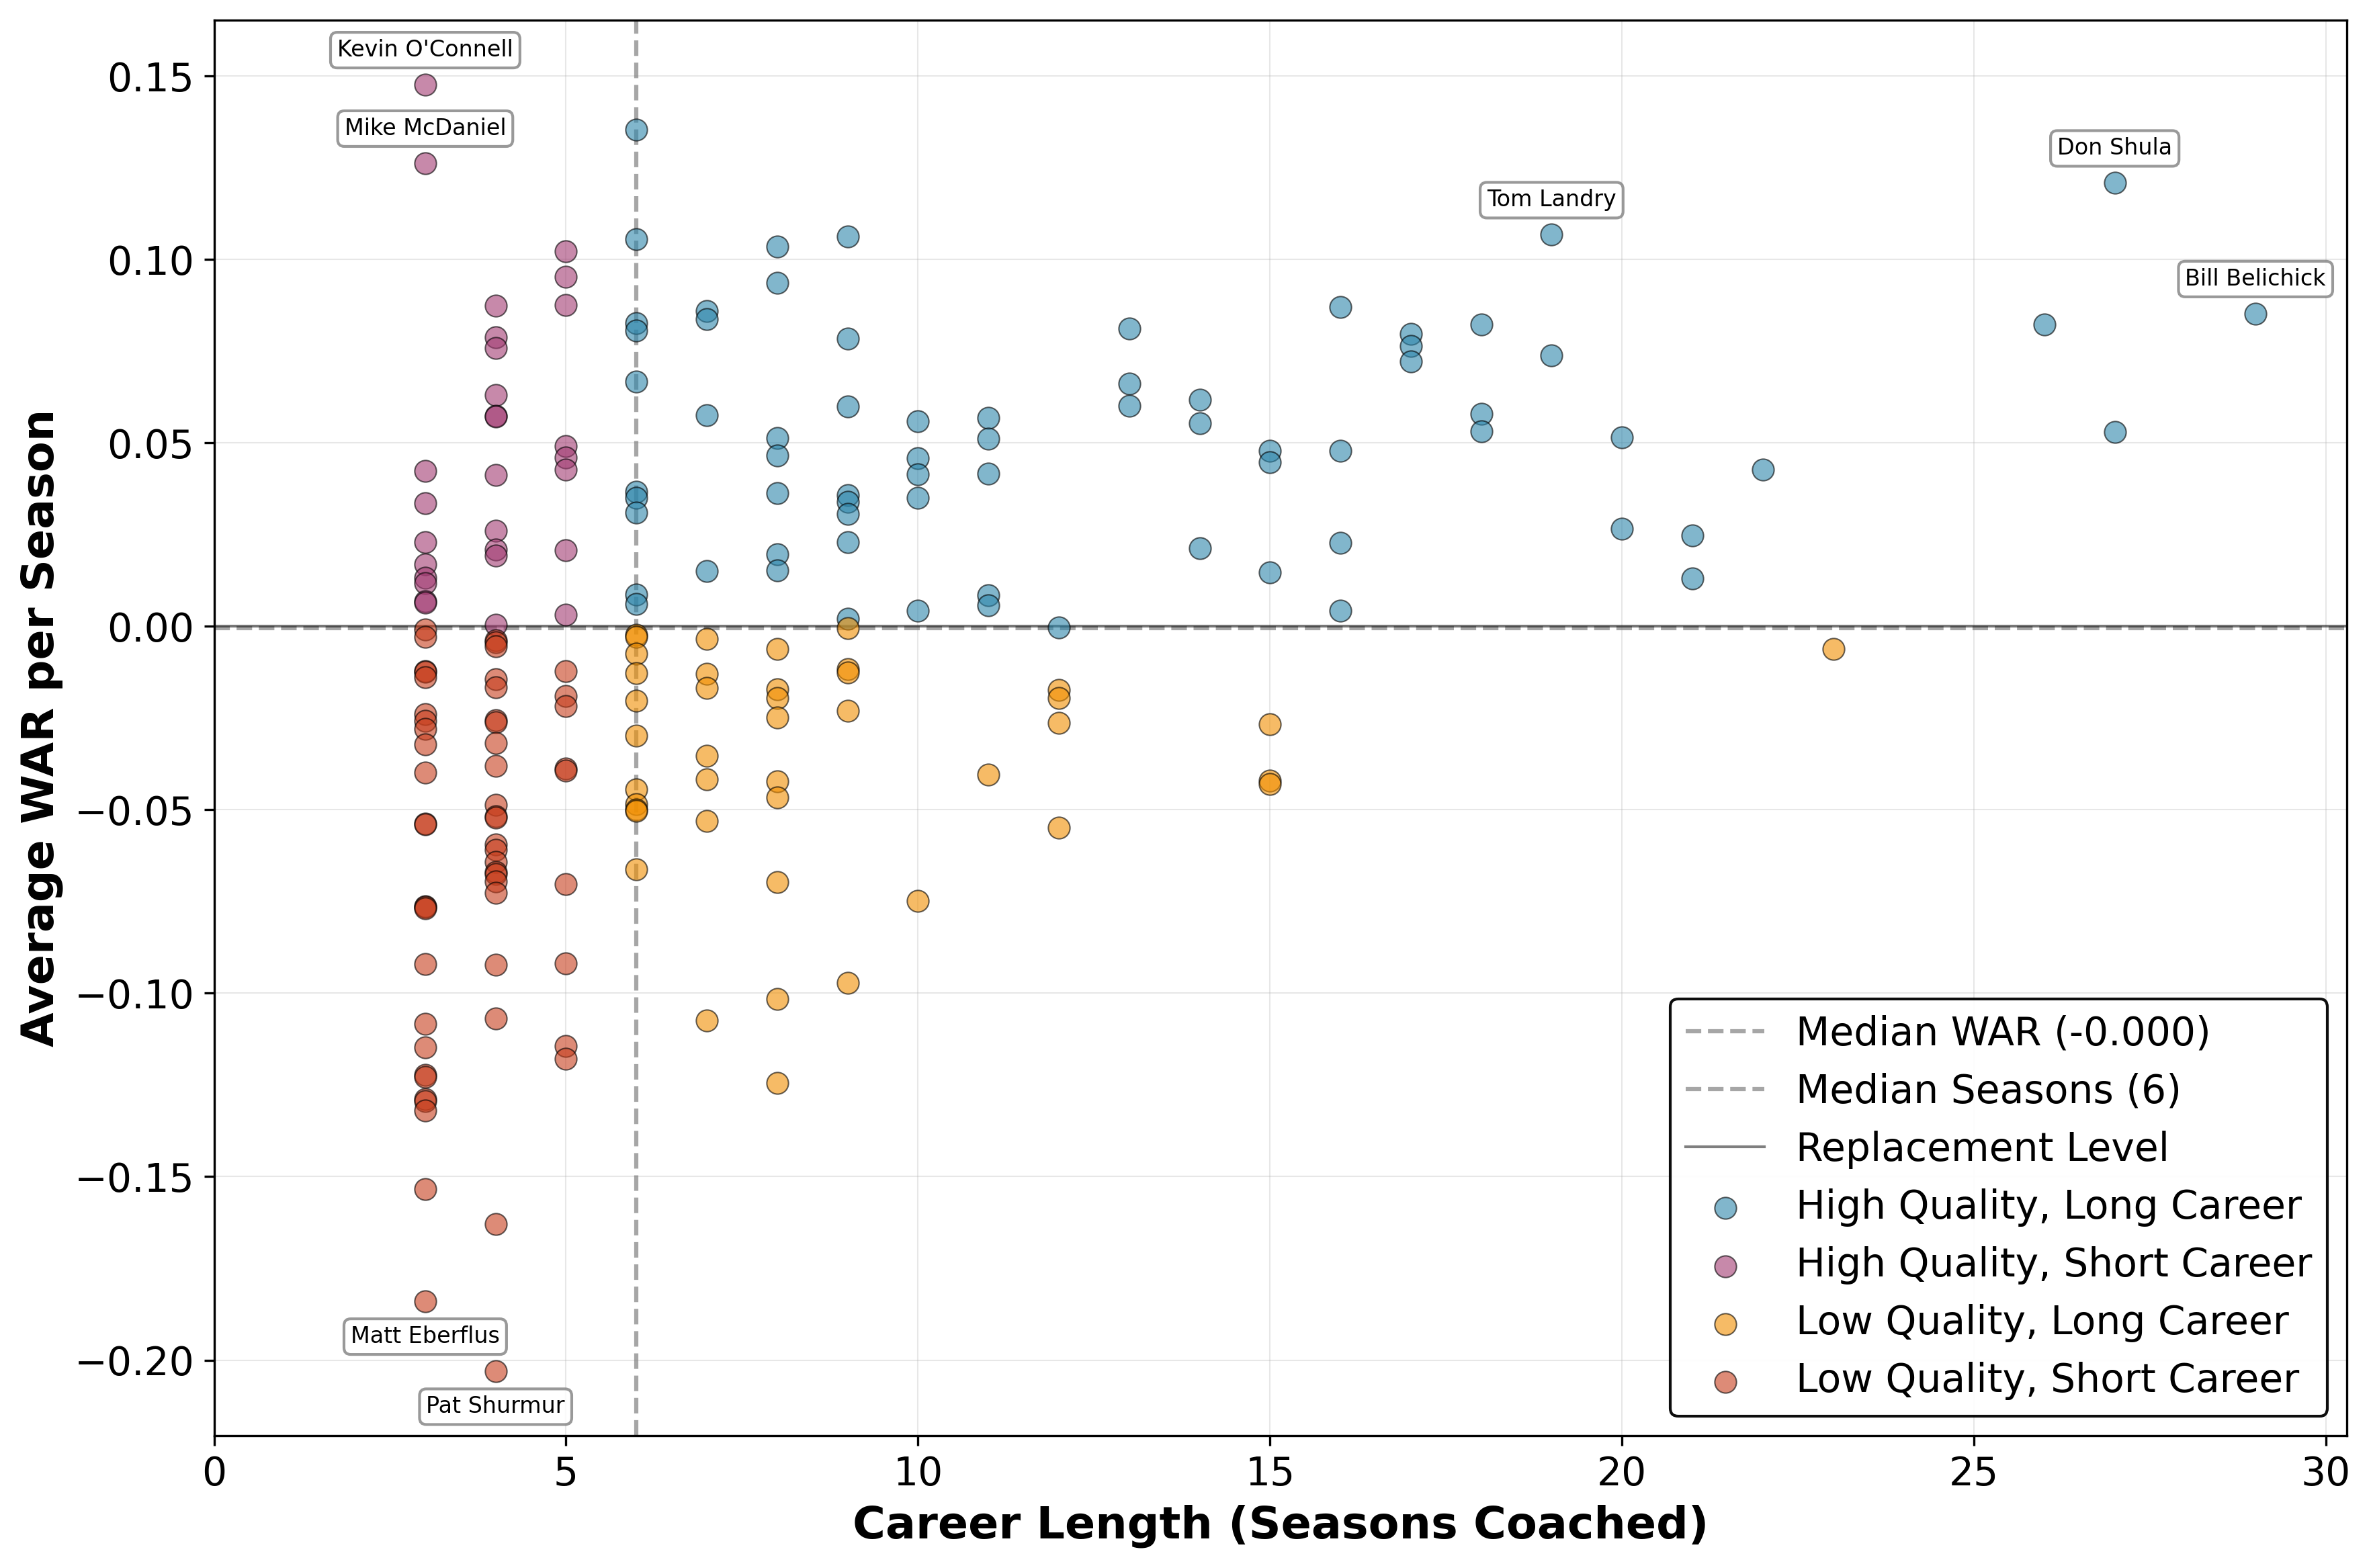
\includegraphics[width=1.0\textwidth]{figures/coach_career_distributions.png}
\caption{Coach WAR Career Distributions}
\label{fig:career_distributions}
\end{figure}

The upper-right and lower-left quadrants show a positive relationship between coaching quality and career length, consistent with organizations retaining successful coaches. However, the lower-right quadrant contains coaches with 5+ seasons despite near-zero or negative WAR, suggesting possible suboptimal retention decisions. Context-adjusted evaluation may help identify such cases earlier.

\subsection{Current Coach Analysis}

Figure \ref{fig:2024_coaches_avg} shows the average career WAR per season for 2024 coaches against their career length. Blue markers indicate coaches who were retained into the 2025 season, and red markers indicate coaches who were fired.

\begin{figure}[!ht]
\centering

\includegraphics[width=1.0\textwidth]{figures/coach_2024_matrix.png}
\caption{2024 Head Coach Average WAR per Season versus Career Length}
\label{fig:2024_coaches_avg}
\end{figure}

To examine individual-season performance, Figure~\ref{fig:2024_trajectories} shows cumulative WAR trajectories for these coaches, and Figure~\ref{fig:2024_single_year} highlights each coach's 2024 WAR.

\begin{figure}[!ht]
\centering

\includegraphics[width=1.0\textwidth]{figures/coach_2024_trajectories.png}
\caption{Coach WAR Trajectory for 2024 Head Coaches}
\label{fig:2024_trajectories}
\end{figure}

\begin{figure}[!ht]
\centering

\includegraphics[width=0.85\textwidth]{figures/coach_2024_single_year_bar.png}
\caption{2024 Coach WAR for 2024 Head Coaches}
\label{fig:2024_single_year}
\end{figure}

Figure~\ref{fig:2024_single_year} illustrates that most fired coaches had negative 2024 WAR, consistent with performance-based decisions. Mike McCarthy's positive 2024 WAR (+1.4) despite dismissal suggests that firing decisions may incorporate factors beyond single-season context-adjusted performance\footnote{Analysis conducted October 2025 on 1970--2024 data; the partially complete 2025 season was excluded.}.

\subsection{Offensive versus Defensive Coaches}

A recurring question concerns whether offensive or defensive coaching backgrounds produce more successful head coaches. For this analysis, coaches were classified based on their coordinator or position coaching experience prior to their head coaching appointment. Across the full modern era (1970--2024), defensive-background coaches hold a slight aggregate edge ($p = 0.168$, Cohen's $d = -0.050$), but this aggregate view obscures substantial era-level variation. Table~\ref{tab:background_by_decade} presents average WAR by background and decade, and Table~\ref{tab:background_decade_stats} reports Mann--Whitney $U$ tests with 95\% confidence intervals on the difference.

\begin{table}[!ht]
\caption{Average Coach WAR per Season by Coach Background and Decade}
\label{tab:background_by_decade}
\small
\begin{tabular}{lcccccc}
\toprule
Background & 1970's & 1980's & 1990's & 2000's & 2010's & 2020's \\
\midrule
Offensive & $-$0.57 & +0.31 & $-$0.48 & $-$0.15 & $-$0.01 & +0.26 \\
Defensive & +0.30 & +0.04 & +0.20 & $-$0.07 & +0.06 & $-$0.33 \\
Other & $-$0.13 & +0.01 & +0.47 & --- & --- & --- \\
\midrule
\multicolumn{7}{l}{\textit{Delta, 2020's vs 1970's}} \\
Offensive & \multicolumn{6}{l}{+0.83} \\
Defensive & \multicolumn{6}{l}{$-$0.63} \\
\bottomrule
\end{tabular}
\end{table}

\begin{table}[!ht]
\caption{Mann-Whitney U Test comparing Coaching Backgrounds by Decade. 95\% CIs are Welch's $t$-intervals on the difference in means (Offensive $-$ Defensive).}
\label{tab:background_decade_stats}
\tiny
\begin{tabular}{lcccccc}
\toprule
Metric & 1970's & 1980's & 1990's & 2000's & 2010's & 2020's \\
\midrule
Sample Size (O/D) & 34/21 & 30/22 & 33/28 & 40/37 & 42/33 & 33/20 \\
Seasons (O/D) & 87/82 & 146/83 & 143/126 & 152/151 & 158/135 & 92/56 \\
Mean WAR (O/D) & $-$0.571/+0.298 & +0.311/+0.042 & $-$0.482/+0.202 & $-$0.148/$-$0.072 & $-$0.006/+0.058 & +0.260/$-$0.332 \\
Difference (O $-$ D) & $-$0.869 & +0.269 & $-$0.684 & $-$0.077 & $-$0.063 & +0.592 \\
95\% CI & [$-$1.45, $-$0.29] & [$-$0.28, +0.82] & [$-$1.13, $-$0.24] & [$-$0.49, +0.34] & [$-$0.52, +0.40] & [$-$0.05, +1.24] \\
U-statistic & 2676 & 6303 & 7300 & 11342 & 10547 & 2981 \\
p-value & 0.005 & 0.613 & 0.007 & 0.861 & 0.871 & 0.110 \\
Significance & Highly Sig. & --- & Highly Sig. & --- & --- & --- \\
\bottomrule
\end{tabular}
\end{table}

In the 1970s, defensive-background coaches held a significant advantage: the offensive-minus-defensive difference was $-$0.87 wins per season (95\% CI: [$-$1.45, $-$0.29], $p = 0.005$). By the 2000s, the groups were indistinguishable ($-$0.08, 95\% CI: [$-$0.49, $+$0.34], $p = 0.86$). In the 2020s, the direction has reversed, with offensive coaches averaging $+$0.59 WAR per season more than defensive coaches (95\% CI: [$-$0.05, $+$1.24], $p = 0.11$). The 2020s interval includes zero, indicating that this reversal, while suggestive, has not yet reached conventional significance levels with the available sample. However, if the current performance differential persists through the remainder of the decade, the roughly doubled sample size would yield a projected $p \approx 0.02$, reaching conventional significance.

Cumulatively, defensive coaches have declined by 0.63 WAR per season from the 1970s to 2020s, while offensive coaches have improved by 0.83 over the same period.

\subsection{WAR Persistence and Scheme Obsolescence}

Coaching performance is unstable from year to year. Analyzing 1,163 consecutive season pairs from 1970--2023, Year N coaching WAR explains only 7.3\% of the variance in Year N+1 performance (Figure \ref{fig:war_persistence}). Elite coaches averaging +2.50 WAR in Year N regress dramatically to just +0.61 in Year N+1, losing $\sim$76\% of their advantage. In contrast, the worst-performing coaches at -2.57 WAR improve substantially to -1.36 WAR when implementing a 10th percentile penalty for being terminated (Figure \ref{fig:war_quintiles}).

\begin{figure}[!ht]
\centering
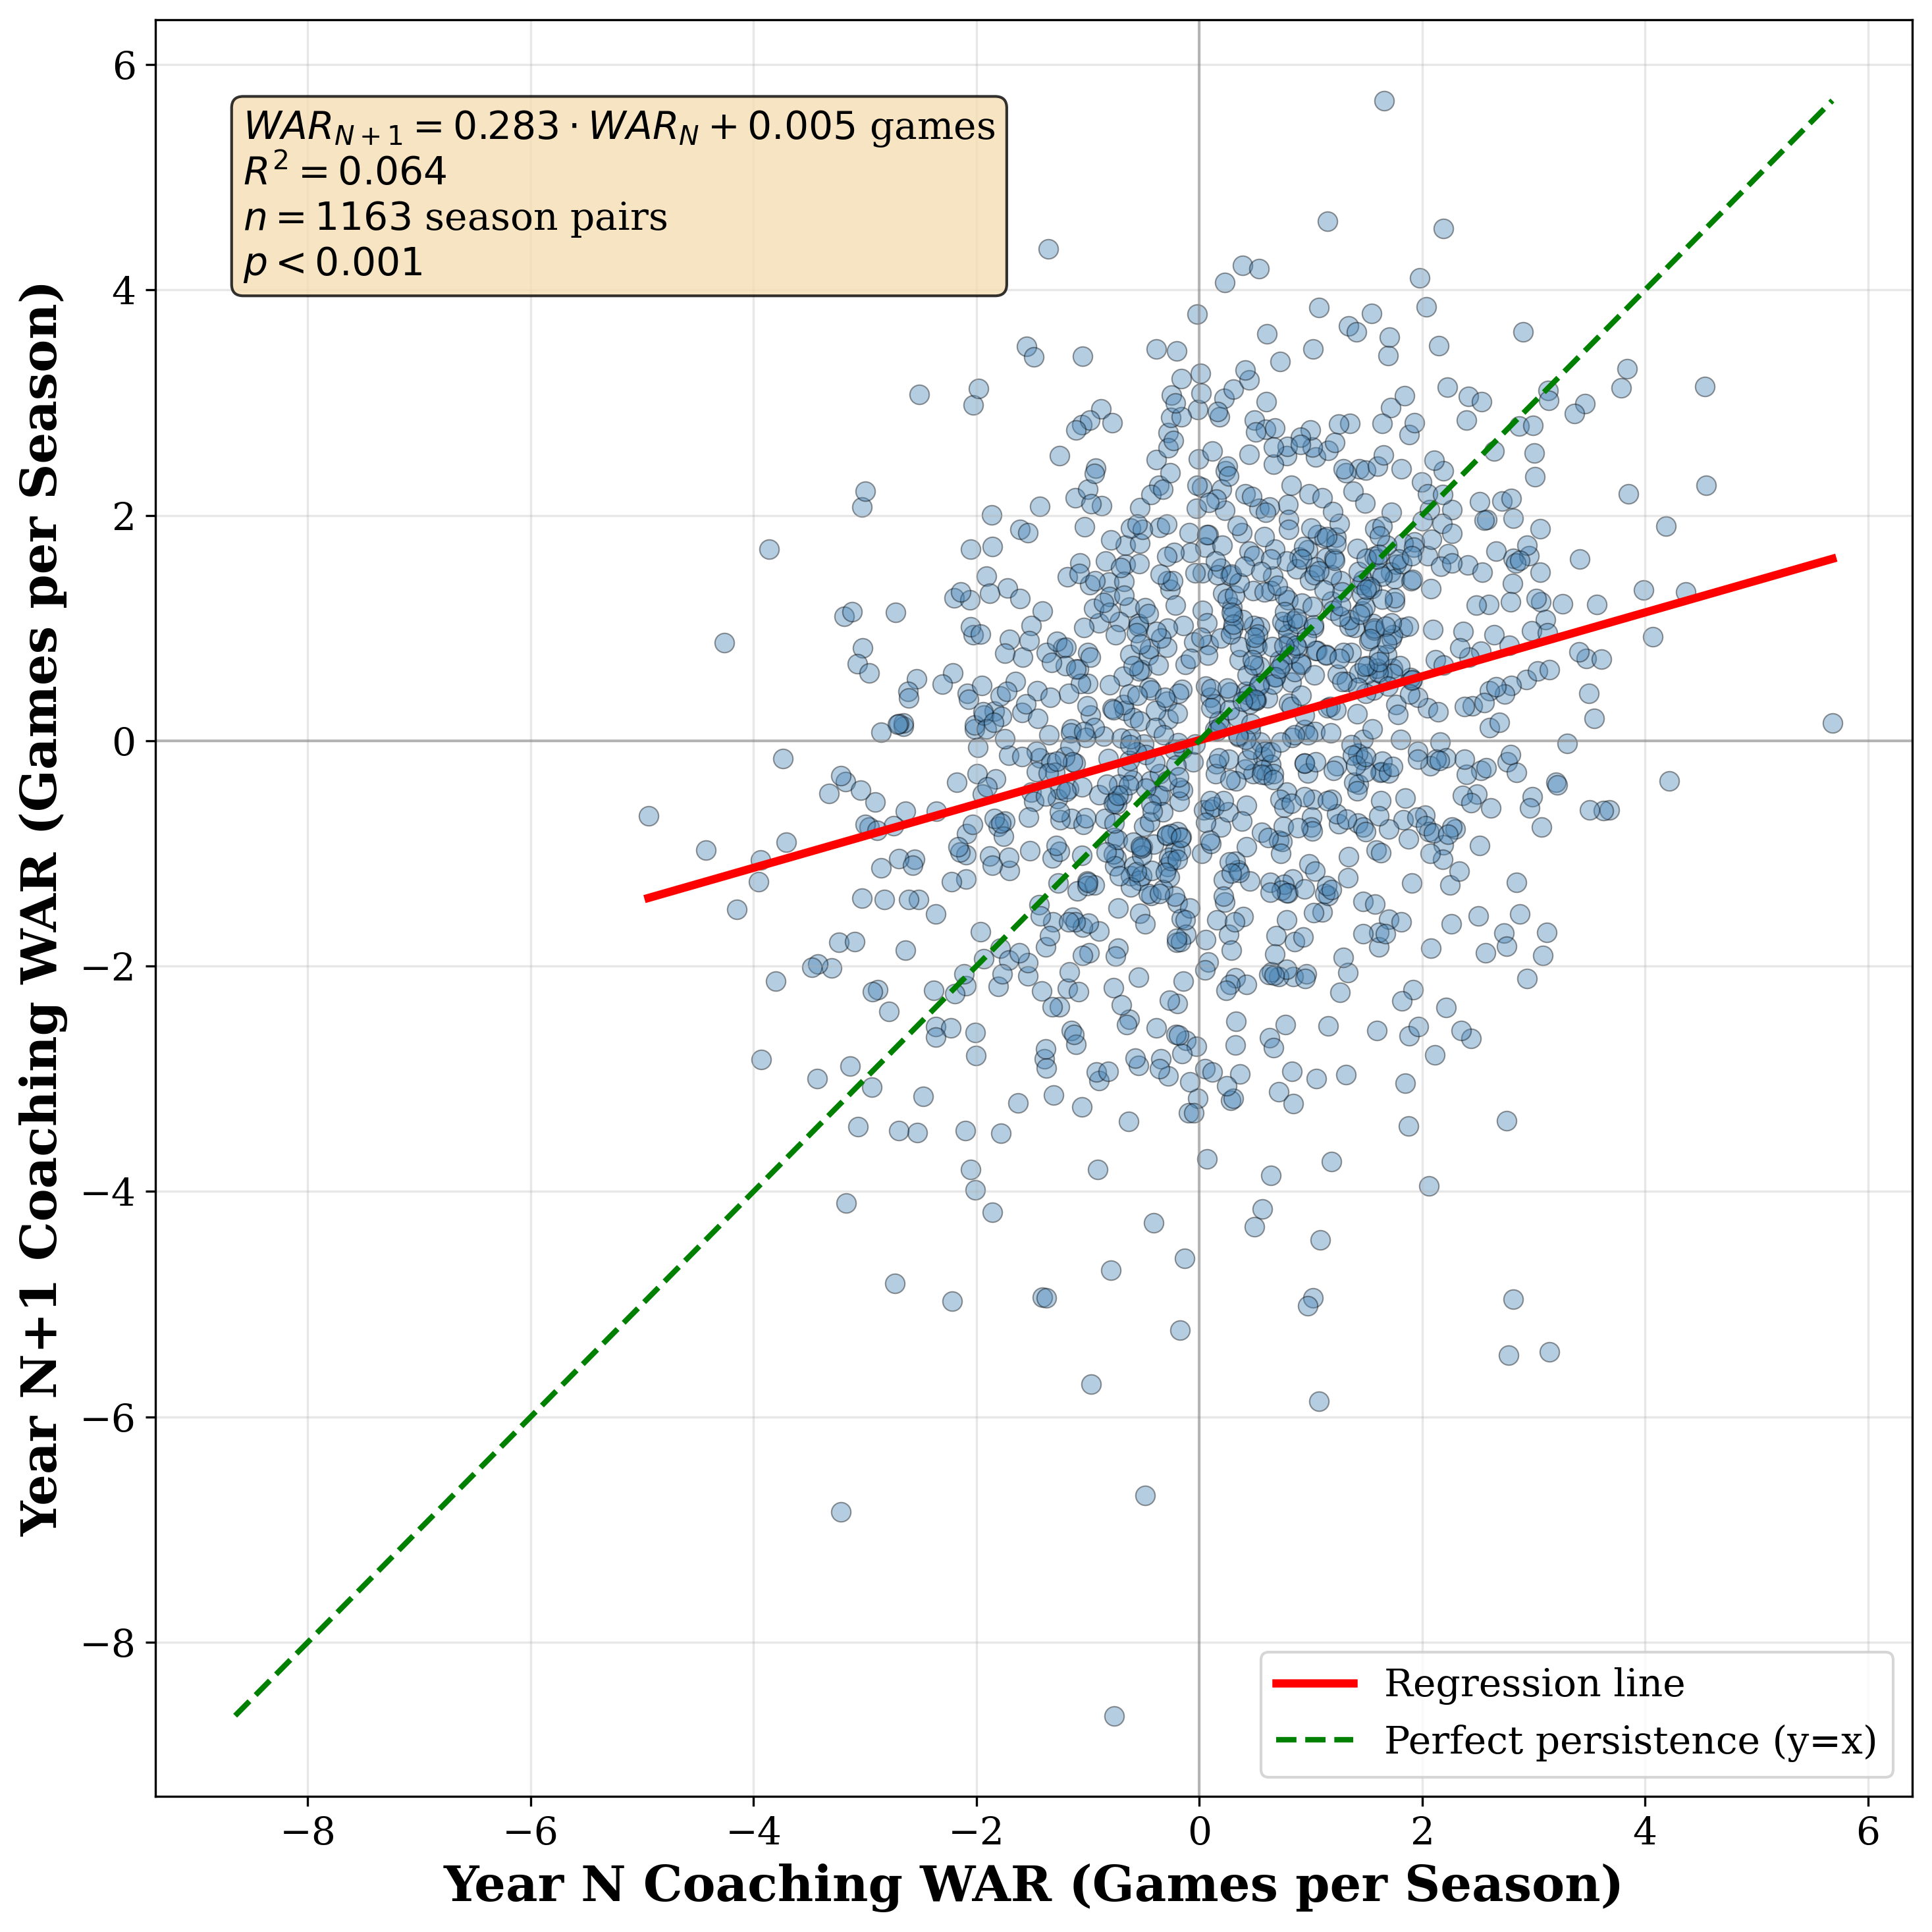
\includegraphics[width=0.8\textwidth]{figures/coaching_war_persistence_scatter.png}
\caption{Coach WAR in Year N+1 vs. Year N (persistence)}
\label{fig:war_persistence}
\end{figure}

\begin{figure}[!ht]
\centering
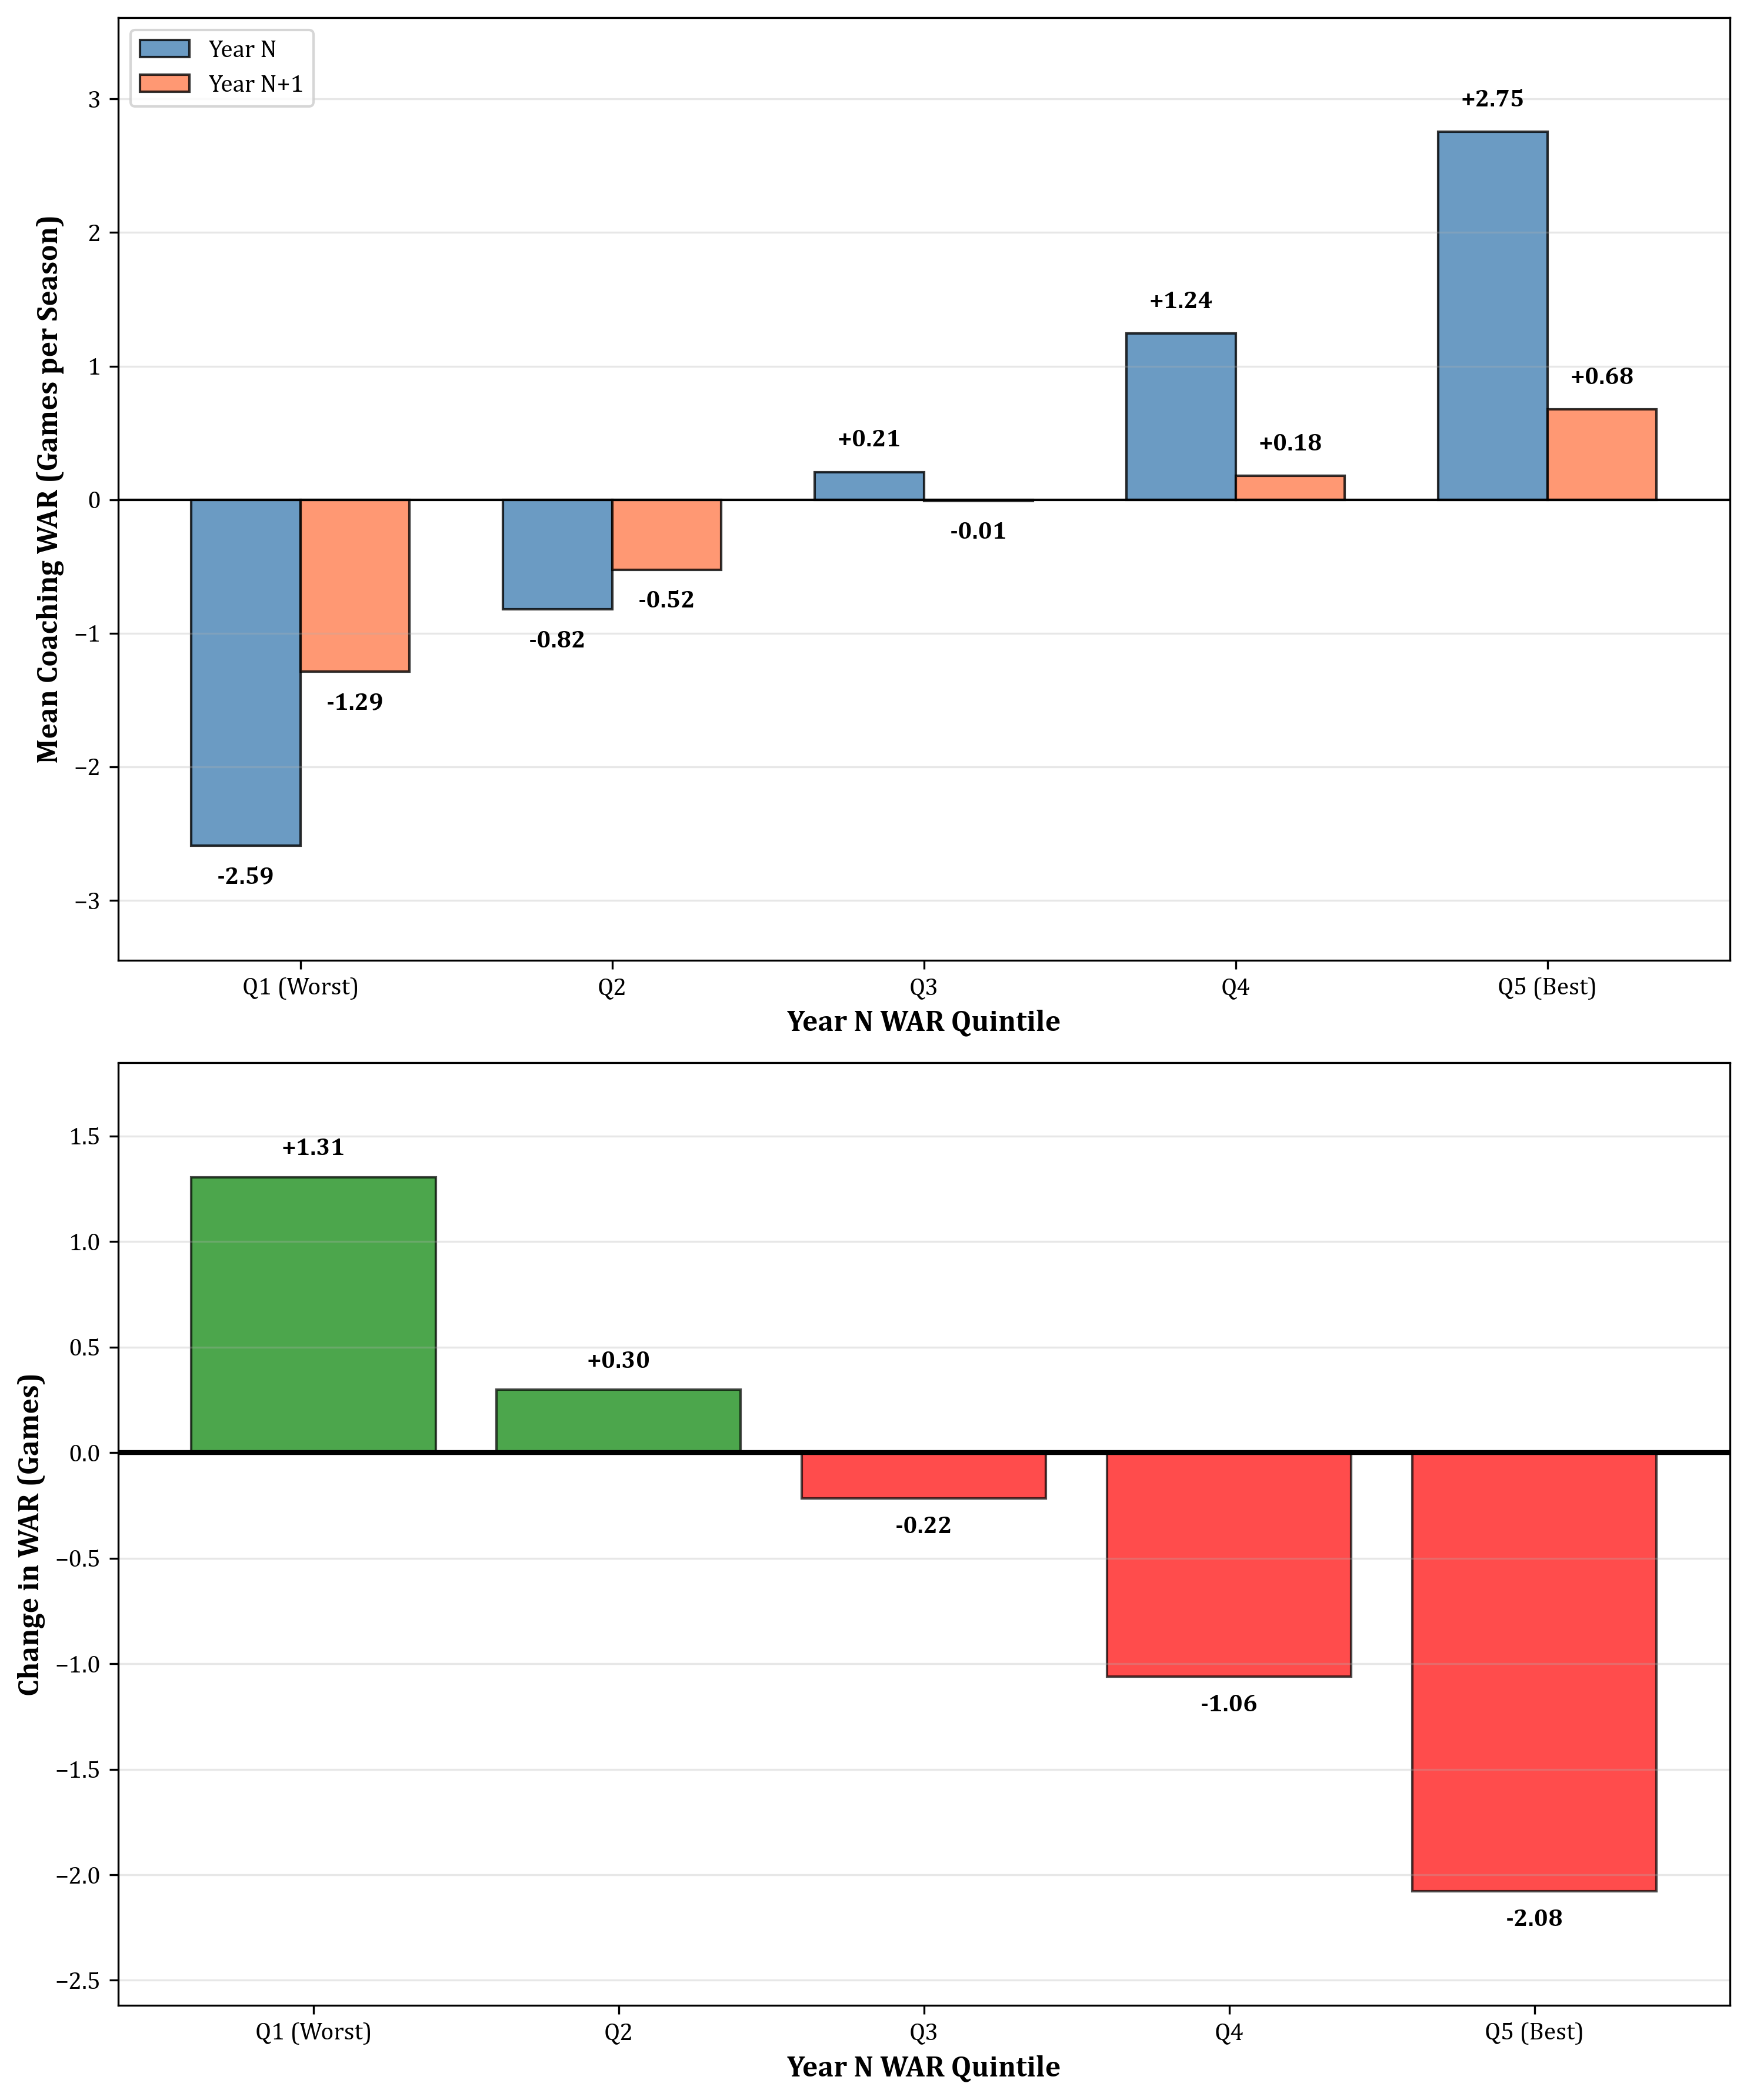
\includegraphics[width=0.95\textwidth]{figures/coaching_regression_to_mean_survivorship_adjusted.png}
\caption{Mean Coach WAR in Year N and Year N+1 by Quintile}
\label{fig:war_quintiles}
\end{figure}

This volatility contrasts sharply with raw winning percentage, which shows nearly double the year-to-year stability (R$^2$ = 0.137, Appendix D, Figure \ref{fig:winpct_persistence}). Winning percentage likely captures persistent organizational advantages, such as market size, ownership stability, and accumulated roster talent, that carry forward regardless of coaching. The coach-specific contribution, by contrast, fluctuates, as what worked last season often doesn't work this season. This represents empirical evidence for scheme obsolescence: coaching innovations that produce short-term advantages are quickly studied, copied, or countered by opposing coaching staffs, causing the advantage to dissipate. In a league where all 32 teams share extensive game film and compete for the same coordinators and assistants, tactical edges diffuse rapidly through the competitive environment.

The instability is not uniform across coaching backgrounds. While both offensive and defensive coaches show similar single-year persistence ($R^2 = 0.064$ and $0.092$ respectively), multi-year averaging reveals a divergence. At a 2-year horizon, defensive coaches' predictive power approximately doubles to $R^2 = 0.180$, while offensive coaches remain flat at $R^2 = 0.069$. This difference is statistically significant (Fisher's $Z$ $p = 0.009$; Appendix~E, Figure~\ref{fig:war_persistence_background} and Table~\ref{tab:war_multiyear_persistence}). At three-year horizons, the gap persists ($p = 0.020$). These patterns suggest that offensive schemes may depreciate more rapidly than defensive approaches, consistent with the notion that offensive innovations are more easily studied and countered from game film.

\subsection{Limitations and the ``Franchise Quarterback Effect''}

Tables \ref{tab:top_single_season} and \ref{tab:bottom_single_season} show the top and bottom 10 single-season WAR instances in the modern era.

\begin{table}[!ht]
\caption{Top 10 Single-Season WAR Instances. Model residual standard error: $\pm$2.0 wins per season.}
\label{tab:top_single_season}
\small
\begin{tabular}{clllccc}
\toprule
Rank & Team & Year & Coach & Actual Win \% & Replacement Win \% & WAR \\
\midrule
1 & CHI & 1987 & Mike Ditka & 0.733 & 0.293 & +7.0 \\
2 & WAS & 1982 & Joe Gibbs & 0.889 & 0.514 & +6.0 \\
3 & CLT & 2009 & Jim Caldwell & 0.875 & 0.501 & +6.0 \\
4 & RAI & 1976 & John Madden & 0.929 & 0.624 & +4.9 \\
5 & DET & 2024 & Dan Campbell & 0.882 & 0.583 & +4.8 \\
6 & NYG & 1986 & Bill Parcells & 0.875 & 0.576 & +4.8 \\
7 & NWE & 2007 & Bill Belichick & 1.000 & 0.707 & +4.7 \\
8 & MIA & 1972 & Don Shula & 1.000 & 0.709 & +4.7 \\
9 & RAI & 1982 & Tom Flores & 0.889 & 0.598 & +4.7 \\
10 & SFO & 1987 & Bill Walsh & 0.867 & 0.579 & +4.6 \\
\bottomrule
\end{tabular}
\end{table}

\begin{table}[!ht]
\caption{Bottom 10 Single-Season WAR Instances. Model residual standard error: $\pm$2.0 wins per season.}
\label{tab:bottom_single_season}
\small
\begin{tabular}{clllccc}
\toprule
Rank & Team & Year & Coach & Actual Win \% & Replacement Win \% & WAR \\
\midrule
1 & ATL & 2020 & Dan Quinn & 0.000 & 0.528 & $-$8.4 \\
2 & PHI & 1971 & Jerry Williams & 0.000 & 0.438 & $-$7.0 \\
3 & CIN & 1996 & David Shula & 0.143 & 0.581 & $-$7.0 \\
4 & SEA & 1982 & Jack Patera & 0.000 & 0.419 & $-$6.7 \\
5 & HTX & 2020 & Bill O'Brien & 0.000 & 0.391 & $-$6.3 \\
6 & CLT & 1991 & Ron Meyer & 0.000 & 0.379 & $-$6.1 \\
7 & CLT & 1972 & Don McCafferty & 0.200 & 0.541 & $-$5.5 \\
8 & RAM & 2008 & Scott Linehan & 0.000 & 0.337 & $-$5.4 \\
9 & CIN & 1971 & Paul Brown & 0.286 & 0.616 & $-$5.3 \\
10 & WAS & 2013 & Mike Shanahan & 0.188 & 0.514 & $-$5.2 \\
\bottomrule
\end{tabular}
\end{table}

The highest single-season WAR values reveal an important limitation. Four of the top 10 single-season values coincide with elite quarterback play (Tom Brady in 2007, Peyton Manning in 2009, Joe Montana in 1987, Bob Griese in 1972). This ``franchise quarterback effect'' reflects the inherent challenge of isolating coaching contributions: elite quarterbacks and elite coaching are rarely independent. While the framework controls for roster quality through player age, experience, and positional spending, it cannot fully disentangle whether a coach maximizes quarterback talent or whether an elite quarterback elevates apparent coaching performance. The remaining top-10 entries (Dan Campbell 2024, Mike Ditka 1987, John Madden 1976, Bill Parcells 1986, Tom Flores 1982, Joe Gibbs 1982) occurred without consensus elite quarterbacks, indicating the framework captures coaching performance beyond quarterback quality. Career-average analysis with confidence intervals (Tables~\ref{tab:top_coaches}--\ref{tab:bottom_coaches}) naturally mitigates single-season noise.

Bill Walsh appears in the top-10 single-season list (+4.6 WAR, 1987), yet his first season (1979, 2--14) produced deeply negative WAR, illustrating both genuine coaching development---Walsh's early struggles gave way to a dynasty---and the inherent variability in single-season estimates. The model residual standard error of $\pm$2.0 wins per season (Section~3.5) indicates that individual-season WAR values carry substantial uncertainty. Career averages with confidence intervals, as presented in Tables~\ref{tab:top_coaches}--\ref{tab:bottom_coaches}, provide more reliable assessments and should be preferred for evaluation purposes.

At the opposite extreme, several bottom-10 entries involve coaches who were winless before a midseason firing. Our approach scales partial seasons to 16 games, which may overstate negative impact, though a midseason dismissal is itself a meaningful performance signal.

Additional limitations warrant consideration. First, while the model controls for roster quality through age, experience, turnover, and salary allocation, these proxy measures cannot fully capture player talent; teams with similar demographic profiles may differ substantially in talent level. Second, organizational factors beyond our data---ownership stability, drafting competence, facility quality---likely influence outcomes but remain unobserved. Third, the model's $\pm$2.0-win residual SE means that single-season WAR differences smaller than approximately 4 wins may not be distinguishable from noise.

\subsection{Practical Applications}

Context-adjusted coaching evaluation may inform hiring, retention, and contract decisions by separating coaching performance from inherited roster quality. For example, a coach with a .500 record but consistently positive WAR may be undervalued relative to a coach with a .600 record who inherited superior talent. Similarly, retention decisions benefit from objective performance baselines: cumulative negative WAR over multiple seasons, particularly when the confidence interval excludes zero (Table~\ref{tab:bottom_coaches}), provides quantitative evidence that performance deficits are structural rather than circumstantial.

\section{Conclusion}

This paper introduces a counterfactual framework for evaluating NFL head coach performance by comparing actual team outcomes to predictions under replacement-level coaching. The approach extends WAR methodologies previously developed for player evaluation in baseball \citep{baumer2015,brill2024} and football \citep{yurko2019} to the coaching domain, where isolating individual contributions is particularly challenging.

Three principal findings emerge. First, coaching impact is substantial: elite coaches average up to +2.4 WAR per season (95\% CI: [+0.9, +3.9] for the current leader), while the poorest coaches average $-$3.5 (95\% CI: [$-$4.7, $-$2.3]), a spread of approximately 5 wins per season at the 95th-to-5th percentile range. Second, the relative effectiveness of offensive and defensive coaching backgrounds has shifted markedly over the modern era, from a significant defensive advantage in the 1970s ($-$0.87, 95\% CI: [$-$1.45, $-$0.29]) to a suggestive offensive advantage in the 2020s ($+$0.59, 95\% CI: [$-$0.05, $+$1.24]). Third, coaching WAR exhibits low year-to-year persistence ($R^2 = 0.073$), with offensive coaches showing significantly less multi-year persistence than defensive coaches (Fisher's $Z$ $p = 0.009$ at the 2-year horizon).

Several limitations temper these findings. The model residual standard error of $\pm$2.0 wins per season means that individual-season WAR estimates carry substantial uncertainty, and career estimates for short-tenured coaches remain imprecise. The framework cannot fully disentangle coaching from unobserved quarterback talent or organizational quality. Additionally, the train--test $R^2$ gap of 0.16 suggests the model may overfit to training data, though coach-based stratification and Ridge regression validation provide partial reassurance.

Future work could incorporate player-level tracking data \citep{lopez2020} to better separate coaching scheme effects from player execution, extend the framework to coordinator evaluation, or apply ensemble methods to produce model-based uncertainty estimates that complement the empirical intervals reported here.

\section*{Data Availability}

Coaching history data was scraped from Pro Football Reference. Processed data and analysis code are available at \url{https://github.com/jwilliamson7/Coach_WAR} or upon request to the corresponding author. Raw salary cap data from Spotrac is proprietary but processing scripts are provided.

\begin{thebibliography}{99}

\bibitem[Appelman and Cameron(2013)]{appelman2013}
Appelman, D. and Cameron, K. (2013). Unifying replacement level. \emph{FanGraphs Baseball}, 28 March. Available at: https://blogs.fangraphs.com/unifying-replacement-level/

\bibitem[Baseball-Reference.com(n.d.)]{baseballref_war}
Baseball-Reference.com (n.d.). Position player WAR calculations and details. Available at: https://www.baseball-reference.com/about/war\_explained\_position.shtml

\bibitem[Baumer et al.(2015)]{baumer2015}
Baumer, B.S., Jensen, S.T. and Matthews, G.J. (2015). openWAR: an open source system for evaluating overall player performance in major league baseball. \emph{Journal of Quantitative Analysis in Sports}, \textbf{11}(2), pp. 69--84.

\bibitem[Berri et al.(2006)]{berri2006}
Berri, D.J., Schmidt, M.B. and Brook, S.L. (2006). \emph{The Wages of Wins}. Stanford, CA: Stanford University Press.

\bibitem[Brand(2002)]{brand2002}
Brand, M. (2002). Incremental singular value decomposition of uncertain data with missing values. In: \emph{Proceedings of the European Conference on Computer Vision}, pp. 707--720.

\bibitem[Brill and Wyner(2024)]{brill2024}
Brill, R.S. and Wyner, A.J. (2024). Introducing Grid WAR: rethinking WAR for starting pitchers. \emph{Journal of Quantitative Analysis in Sports}, \textbf{20}(4), pp. 293--329.

\bibitem[Chen and Guestrin(2016)]{chen2016}
Chen, T. and Guestrin, C. (2016). XGBoost: a scalable tree boosting system. In: \emph{KDD '16: Proceedings of the 22nd ACM SIGKDD International Conference on Knowledge Discovery and Data Mining}, pp. 785--794.

\bibitem[Deshpande and Jensen(2016)]{deshpande2016}
Deshpande, S.K. and Jensen, S.T. (2016). Estimating an NBA player's impact on his team's chances of winning. \emph{Journal of Quantitative Analysis in Sports}, \textbf{12}(2), pp. 51--72.

\bibitem[Goff and Wisley(2006)]{goff2006}
Goff, B.L. and Wisley, T.L. (2006). Is there a managerial life cycle? Evidence from the NFL. \emph{Managerial and Decision Economics}, \textbf{27}(6), pp. 563--572.

\bibitem[Hadley et al.(2000)]{hadley2000}
Hadley, L., Poitras, M., Ruggiero, J. and Knowles, S. (2000). Performance evaluation of National Football League teams. \emph{Managerial and Decision Economics}, \textbf{21}(2), pp. 63--70.

\bibitem[Lock and Nettleton(2014)]{lock2014}
Lock, D. and Nettleton, D. (2014). Using random forests to estimate win probability before each play of an NFL game. \emph{Journal of Quantitative Analysis in Sports}, \textbf{10}(2), pp. 197--205.

\bibitem[Lopez(2020)]{lopez2020}
Lopez, M.J. (2020). Bigger data, better questions, and a return to fourth down behavior: an introduction to a special issue on tracking data in the National Football League. \emph{Journal of Quantitative Analysis in Sports}, \textbf{16}(2), pp. 73--79.

\bibitem[Palmer and Thorn(1984)]{palmer1984}
Palmer, P. and Thorn, J. (1984). \emph{The Hidden Game of Baseball}. Garden City, NY: Doubleday.

\bibitem[Sabin(2021)]{sabin2021}
Sabin, R. (2021). Estimating player value in American football using plus--minus models. \emph{Journal of Quantitative Analysis in Sports}, \textbf{17}(4), pp. 313--364.

\bibitem[Smith(2008)]{smith2008}
Smith, S. (2008). Total Baseball Ranking: A new method for rating baseball players. \emph{Baseball Reference}. Available at: https://www.baseball-reference.com/about/war\_explained.shtml

\bibitem[Witnauer et al.(2007)]{witnauer2007}
Witnauer, W., Rogers, R. and Saint Onge, J. (2007). Major league baseball career length in the twentieth century. \emph{Population Research and Policy Review}, \textbf{26}(4), pp. 371--386.

\bibitem[Woolner(2002)]{woolner2002}
Woolner, K. (2002). VORP: Value over replacement player. \emph{Baseball Prospectus}. Available at: https://www.baseballprospectus.com

\bibitem[Yurko et al.(2019)]{yurko2019}
Yurko, R., Ventura, S. and Horowitz, M. (2019). nflWAR: a reproducible method for offensive player evaluation in football. \emph{Journal of Quantitative Analysis in Sports}, \textbf{15}(3), pp. 163--183.

\end{thebibliography}

\clearpage

\appendix

\section{Feature Count Across Categories}

\begin{table}[!ht]
\caption{Feature Count Across Categories}
\label{tab:feature_counts}
\begin{tabular}{lcc}
\toprule
Feature Category & Coach Feature? & Number of Features \\
\midrule
Metadata (excluded from training) & No & 2 \\
Salary Cap & No & 19 \\
Roster Turnover & No & 63 \\
Starter Turnover & No & 27 \\
Injury/Availability & No & 37 \\
Player Demographics & No & 44 \\
Penalty/Opponent & No & 7 \\
Draft Capital & No & 29 \\
Coaching Experience & Yes & 7 \\
Prior Team Performance (OC) & Yes & 33 \\
Prior Team Performance (DC) & Yes & 33 \\
Prior Team Performance (HC) & Yes & 66 \\
Target Variable & No & 1 \\
\midrule
\textbf{Total Columns in Dataset} & & \textbf{368} \\
\textbf{Features Used in Training} & & \textbf{365} \\
\bottomrule
\end{tabular}
\end{table}

\clearpage

\section{Selected Hyperparameters for the Final Model}

\begin{table}[!ht]
\caption{Selected Hyperparameters for the Final Model}
\label{tab:hyperparameters}
\begin{tabular}{lc}
\toprule
Hyperparameter & Value \\
\midrule
Objective & reg:squarederror \\
Random State & 42 \\
Number of Estimators & 300 \\
Learning Rate & 0.05 \\
Max Estimator Depth & 2 \\
Gamma & 0 \\
Lambda & 0.1 \\
Alpha & 0.1 \\
Subsample & 0.7 \\
Colsample by Tree & 1.0 \\
Minimum Child Weight & 5 \\
\bottomrule
\end{tabular}
\end{table}

\clearpage

\section{Feature Importance Ranking of Top 20 Features}

\begin{table}[!ht]
\caption{Feature Importance Ranking of Top 20 Features}
\label{tab:feature_importance}
\small
\begin{tabular}{clcl}
\toprule
Rank & Feature Description & Importance & Coach Metric \\
\midrule
1 & Reserve/injured/suspended cap as percentage & 0.031 & No \\
2 & Normalized opponent interceptions thrown & 0.026 & No \\
3 & Normalized passing TDs under HC & 0.024 & Yes \\
4 & Normalized opponent avg pts per drive under HC & 0.023 & Yes \\
5 & Normalized opponent yards allowed under HC & 0.022 & Yes \\
6 & Normalized points scored under HC & 0.022 & Yes \\
7 & Normalized team interceptions thrown & 0.021 & No \\
8 & Normalized scoring percentage under HC & 0.018 & Yes \\
9 & Normalized opponent points scored under HC & 0.017 & Yes \\
10 & Average percentage of games missed by QBs & 0.016 & No \\
11 & Active 53-man roster cap as percentage & 0.015 & No \\
12 & Average experience of all starters & 0.013 & No \\
13 & Number of new QBs added to roster & 0.012 & No \\
14 & New cornerback player rate percentage & 0.010 & No \\
15 & Average age of entire roster & 0.010 & No \\
16 & Number of new TEs added to roster & 0.010 & No \\
17 & Normalized opponent red zone attempts under HC & 0.010 & Yes \\
18 & Normalized 4th down attempts under OC & 0.009 & Yes \\
19 & Average experience of entire roster & 0.009 & No \\
20 & Average experience of offensive linemen & 0.008 & No \\
\bottomrule
\end{tabular}
\end{table}

\clearpage

\section{Win Percentage Persistence}

\begin{figure}[!ht]
\centering

\includegraphics[width=0.8\textwidth]{figures/win_pct_persistence_scatter.png}
\caption{Coach Win Percentage in Year N+1 vs. Year N}
\label{fig:winpct_persistence}
\end{figure}

\clearpage

\section{WAR Persistence by Coach Background}

\begin{figure}[!ht]
\centering
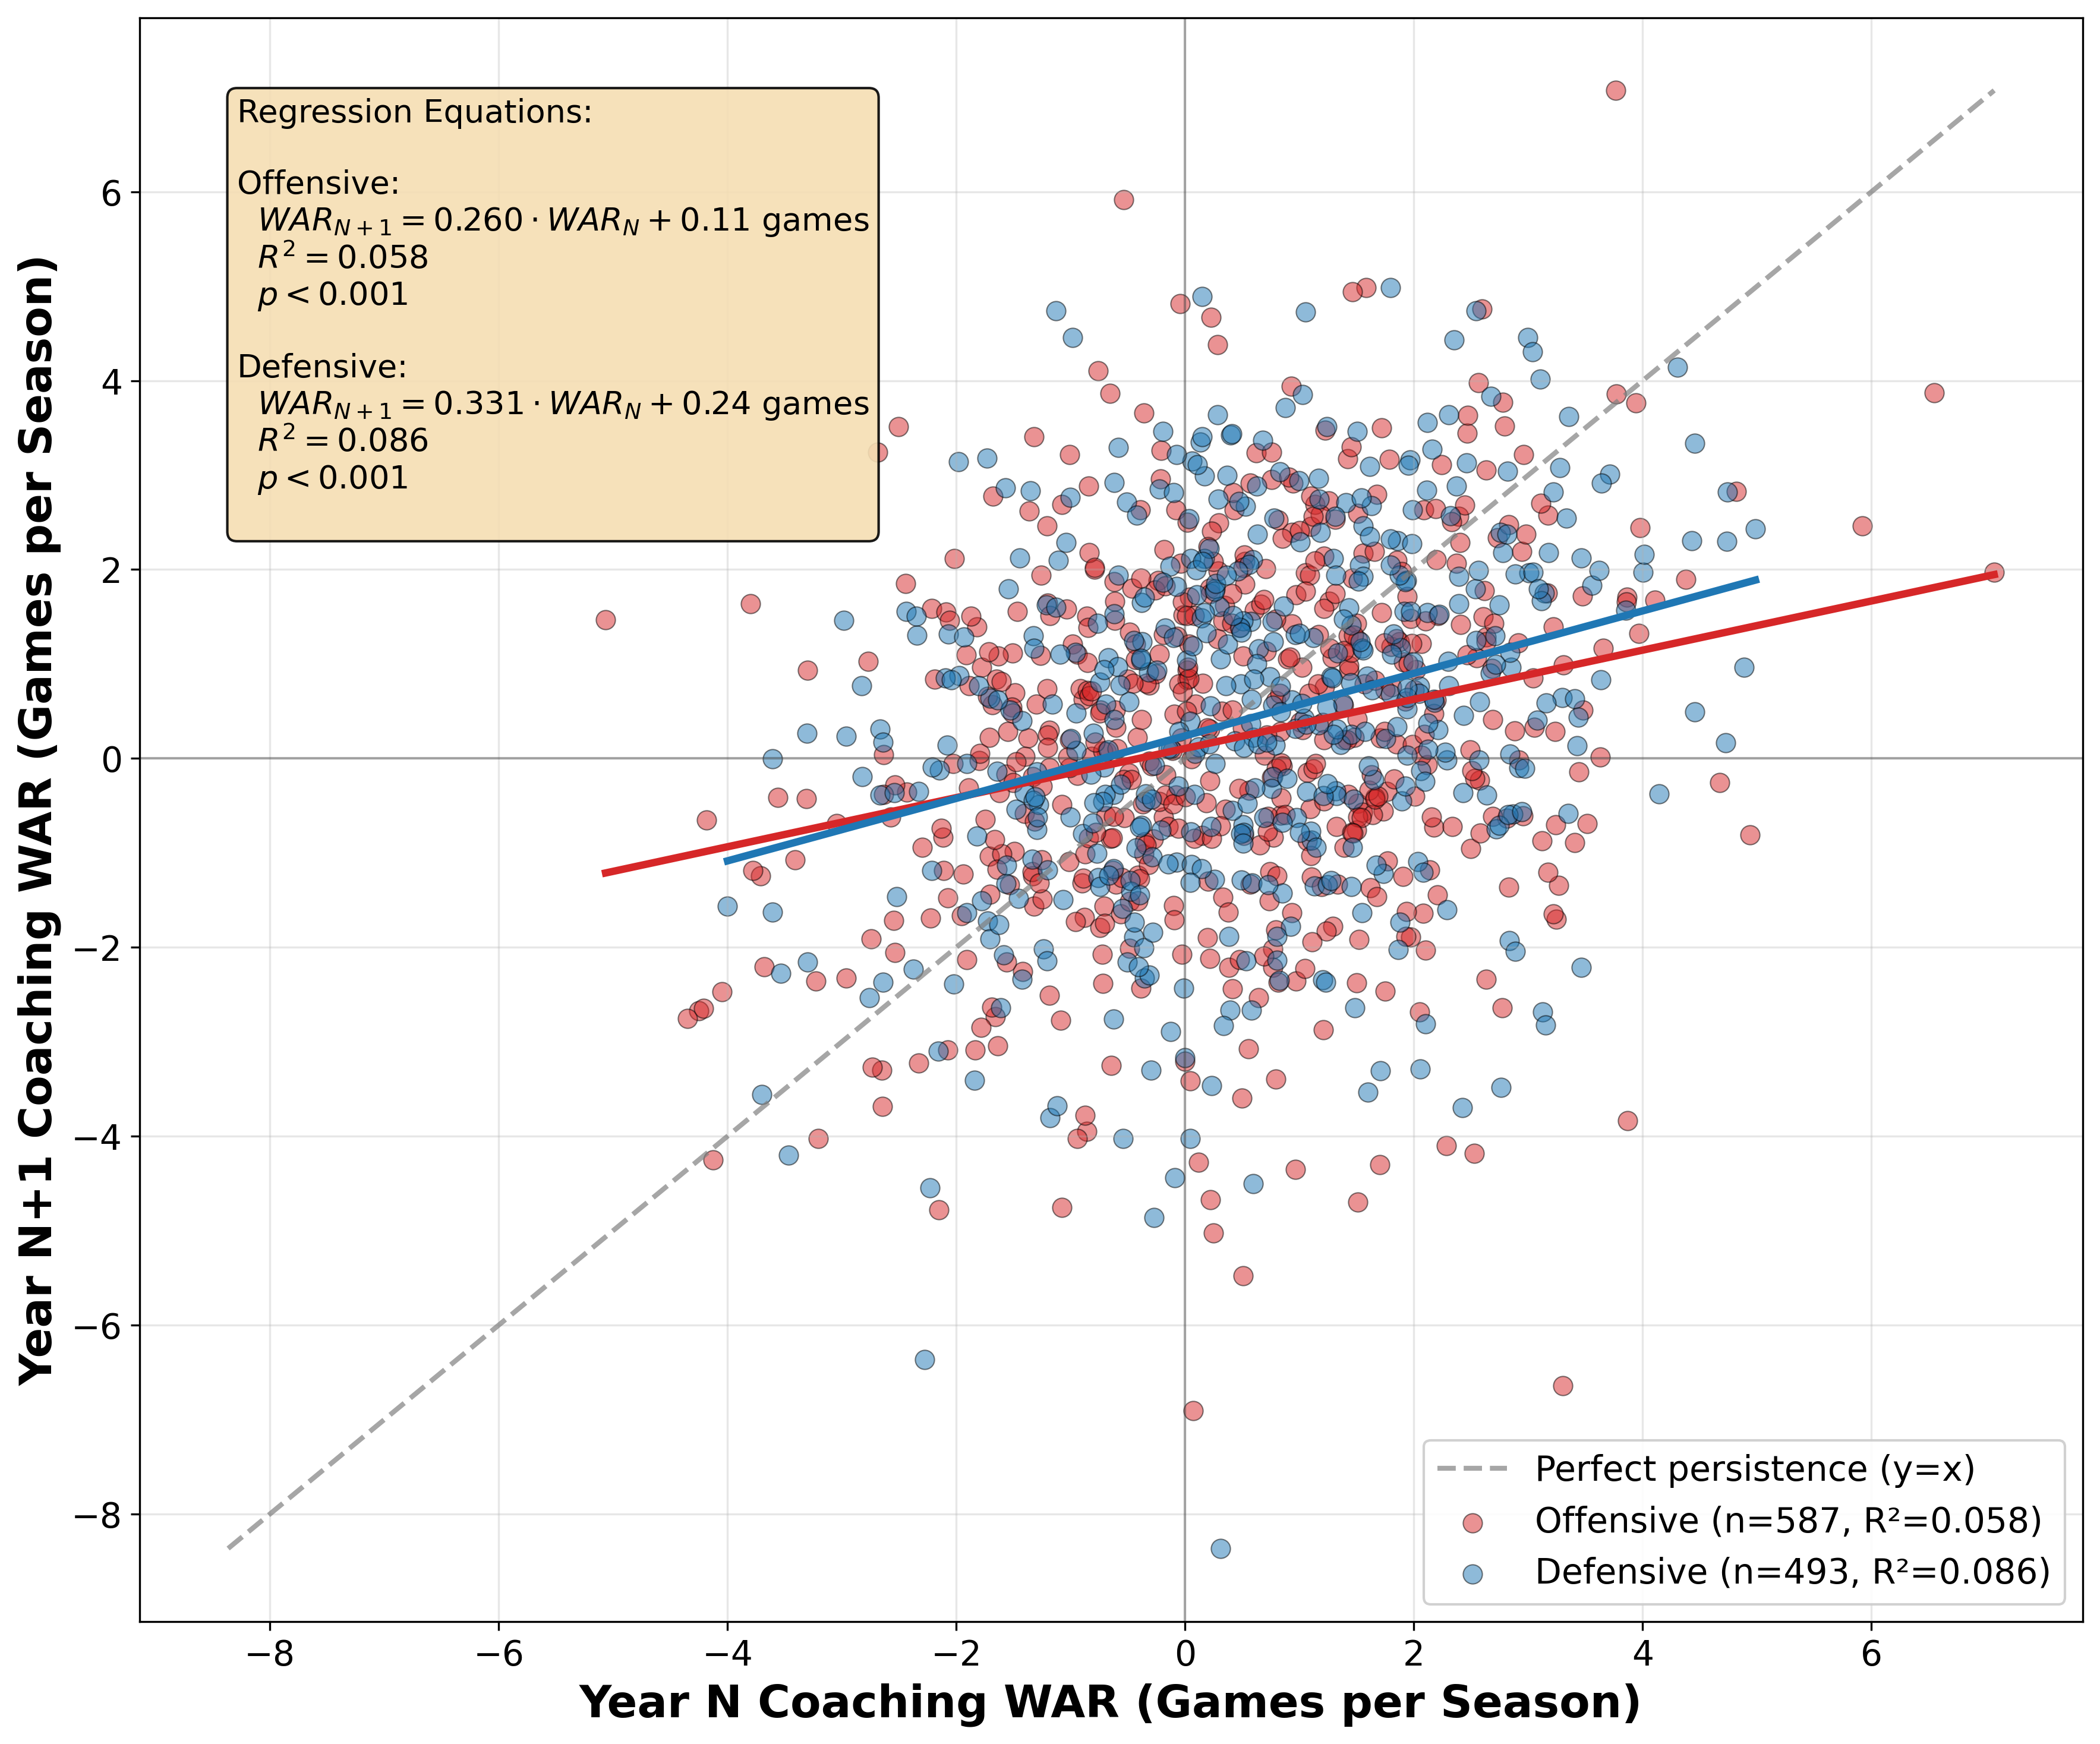
\includegraphics[width=0.8\textwidth]{figures/coaching_war_persistence_by_background.png}
\caption{Coach WAR in Year N+1 vs. Year N by Coach Background}
\label{fig:war_persistence_background}
\end{figure}

\begin{table}[!ht]
\caption{Coaching WAR Persistence by Background and Time Horizon}
\label{tab:war_multiyear_persistence}
\begin{tabular}{lcccccc}
\toprule
 & \multicolumn{2}{c}{\textbf{Offensive}} & \multicolumn{2}{c}{\textbf{Defensive}} & \multicolumn{2}{c}{\textbf{Other}} \\
\cmidrule(lr){2-3} \cmidrule(lr){4-5} \cmidrule(lr){6-7}
\textbf{Time Horizon} & \textbf{R²} & \textbf{p-value} & \textbf{R²} & \textbf{p-value} & \textbf{R²} & \textbf{p-value} \\
\midrule
1-year & 0.064 & <0.001 & 0.092 & <0.001 & 0.032 & 0.103 \\
2-year avg & 0.069 & <0.001 & 0.180 & <0.001 & 0.005 & 0.587 \\
3-year avg & 0.047 & <0.001 & 0.153 & <0.001 & 0.018 & 0.357 \\
4-year avg & 0.038 & 0.004 & 0.135 & <0.001 & 0.019 & 0.429 \\
\bottomrule
\end{tabular}

\smallskip
\footnotesize
Note: Fisher's Z-test for difference in correlations (Offensive vs Defensive): 1-year (p=0.380), 2-year (p=0.009), 3-year (p=0.020), 4-year (p=0.054).
\end{table}

\end{document}
